\anonsection{Цель лабораторной работы}
Целью лабораторной работы №2 является освоение возможностей программы Microsoft Project для определения ресурсов и затрат для проекта. 
Каждое задание лабораторной работы №2 должно выполняться и сохраняться в отдельном файле MS Project.

Команда разработчиков из 16 человек занимается созданием карты города на основе собственного модуля отображения. 
Проект должен быть завершен в течение 6 месяцев. Бюджет проекта: 50 000 рублей.
Лабораторная работа выполнена в Microsoft Project 2019 года, операционная система – Windows 10.

\anonsection{Тренировочное задание}
Вариант по распределению группы -- 4, следовательно, мой вариант для тренировочного задания -- 0.

Требуется для тренировочного задания из прошлой лабораторной работы назначить ресурсы в соответствии с таблицей.

Чтобы смоделировать штат из 10 человек с одинаковой ставкой, был добавлен один ресурс -- человек, но его максимальная загрузка -- 1000\%, что позволяет менять количество работающих человек, меняя лишь проценты.
Материальный ресурс используется для задачи E.
Результат добавления ресурсов в лист ресурсов представлен на рисунке 1:
\FloatBarrier
\begin{figure}[h]	
	\begin{center}
		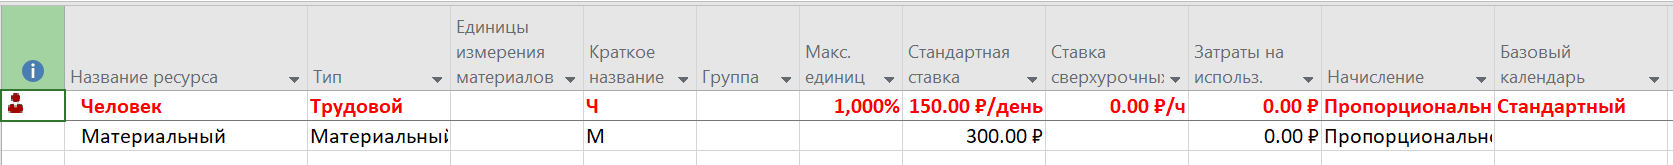
\includegraphics[width=\linewidth]{inc/resurs.png}
	\end{center}
	\captionsetup{justification=centering}
	\caption{Добавление ресурсов}
\end{figure}
\FloatBarrier

Чтобы настроить потребление ресурсов, нужно указать в процентах количество используемых человек (100\% -- 1 человек, 200\% -- 2 человека).
Это можно сделать в меню задачи.
Там же можно настроить и добавление материального ресурса.

Меню представлено на рисунке 2:
\FloatBarrier
\begin{figure}[h]	
	\begin{center}
		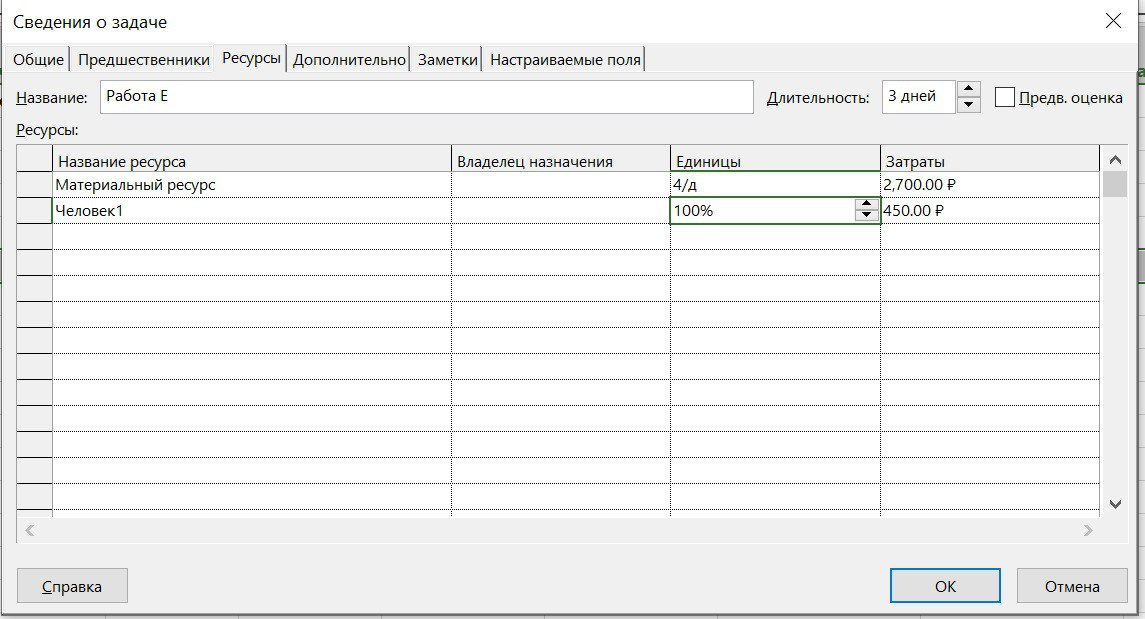
\includegraphics[width=\linewidth]{inc/0-2.jpg}
	\end{center}
	\captionsetup{justification=centering}
	\caption{Меню добавления ресурса к задаче}
\end{figure}
\FloatBarrier

Итоговый лист задач представлен на рисунке 3:
\FloatBarrier
\begin{figure}[h]	
	\begin{center}
		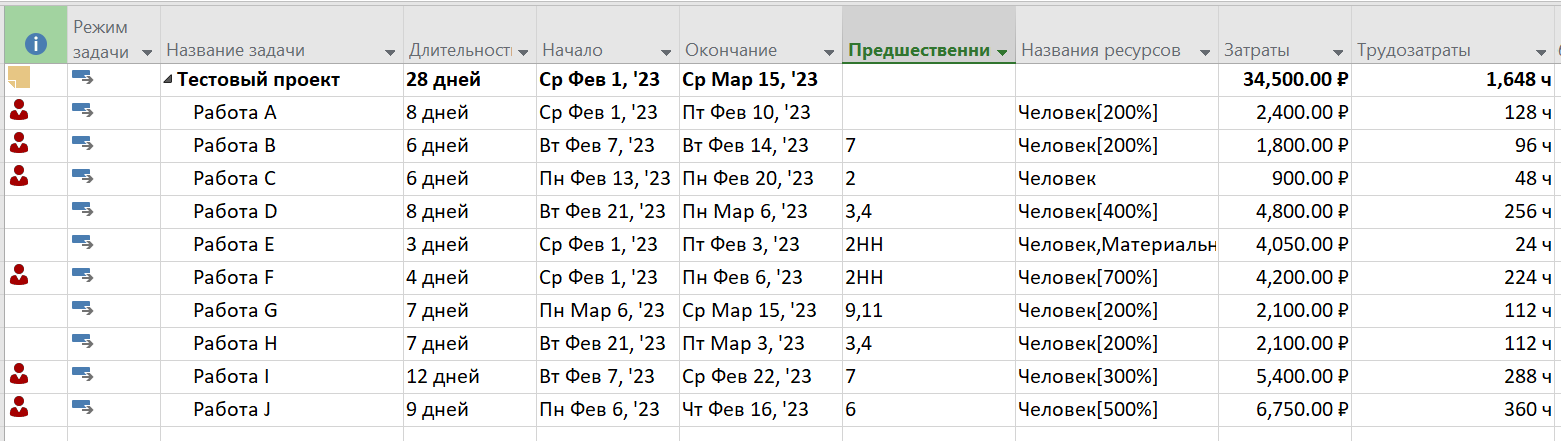
\includegraphics[width=\linewidth]{inc/result.png}
	\end{center}
	\captionsetup{justification=centering}
	\caption{Лист задач}
\end{figure}
\FloatBarrier

Результат сохранён в отдельном файле \textbf{test.mpp}.
\newpage

\anonsection{Задание 1}
В этом задании требуется создать список ресурсов в соответствии с таблицей из методического пособия.
Во вкладке Вид можно изменить вид с \textit{Диаграмма Ганта} на \textit{Лист ресурсов}.
 
В ней можно добавлять новые ресурсы, нажимая соответствующую кнопку или вручную добавляя записи в таблицу.
Полученный результат представлен на рисунке 1:
\FloatBarrier
\begin{figure}[h]	
	\begin{center}
		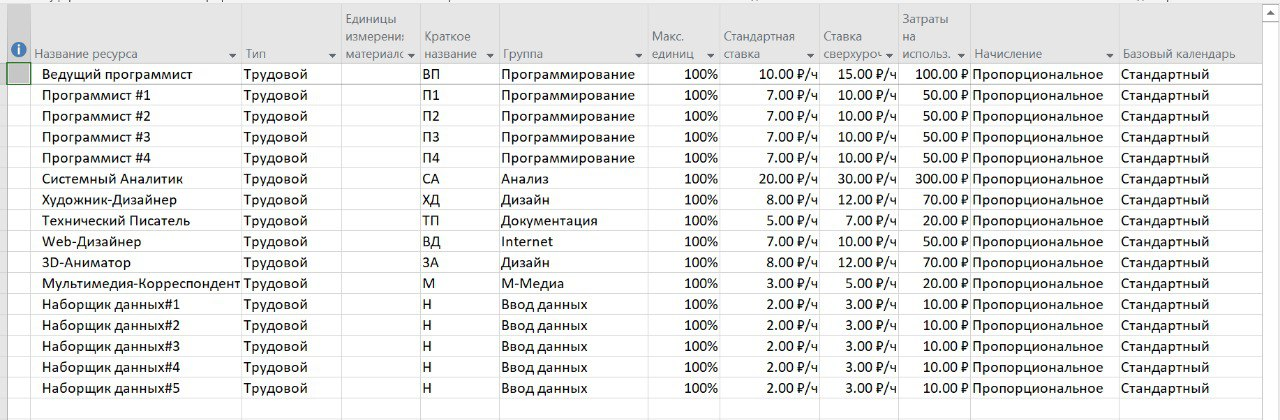
\includegraphics[width=\linewidth]{inc/1-1.jpeg}
	\end{center}
	\captionsetup{justification=centering}
	\caption{Выполнение задания 1}
\end{figure}
\FloatBarrier

Столбец \textit{Единицы измерения материалов} не использовался. 
Календарь для всех ресурсов выбран по-умолчанию – стандартный. 
Календарь проекта также был основан на стандартном календаря, но с учётом выходных и праздников.
Ресурсы впоследствии учитывались также – с учётом графика рабочих дней в Российской Федерации.

В столбце \textit{Начисления} использовалось значение \textbf{Пропорционально}: затраты рассчитываются и списываются за каждый день использования ресурса.

\anonsection{Задание 2}
В этом задании требуется назначить на каждое задание из лабораторной работы 1 созданные в предыдущем задании ресурсы в соответствии с таблицей из методического пособия.

Это можно сделать как через полноценное меню каждой задачи, так и выбрав из выпадающего списка в столбце \textit{Назначение ресурсов} ресурсы для каждой задачи, перейдя в пункт \textit{Вид} -> \textit{Лист Задач}.
В этой же таблице можно задать фиксированные затраты для задач, выбрав пункт \textit{Фиксированные затраты}.
Для того, чтобы имитировать аренду сервера, был добавлен новый ресурс – \textbf{Сервер}, для которого добавлена стандартная ставка 2 руб/час, а календарь выбран \textbf{24 часа}.
Добавление нового ресурса изображено на рисунке 2:
\FloatBarrier
\begin{figure}[h]	
	\begin{center}
		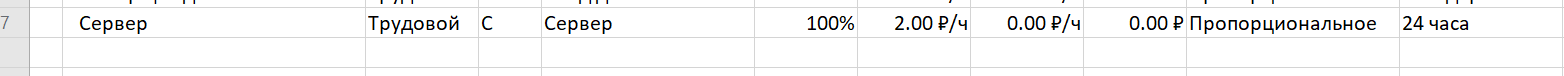
\includegraphics[width=\linewidth]{inc/2.png}
	\end{center}
	\captionsetup{justification=centering}
	\caption{Выполнение задания 2-1}
\end{figure}
\FloatBarrier

Итоговый результат представлен на рисунке 3:
\FloatBarrier
\begin{figure}[h]	
	\begin{center}
		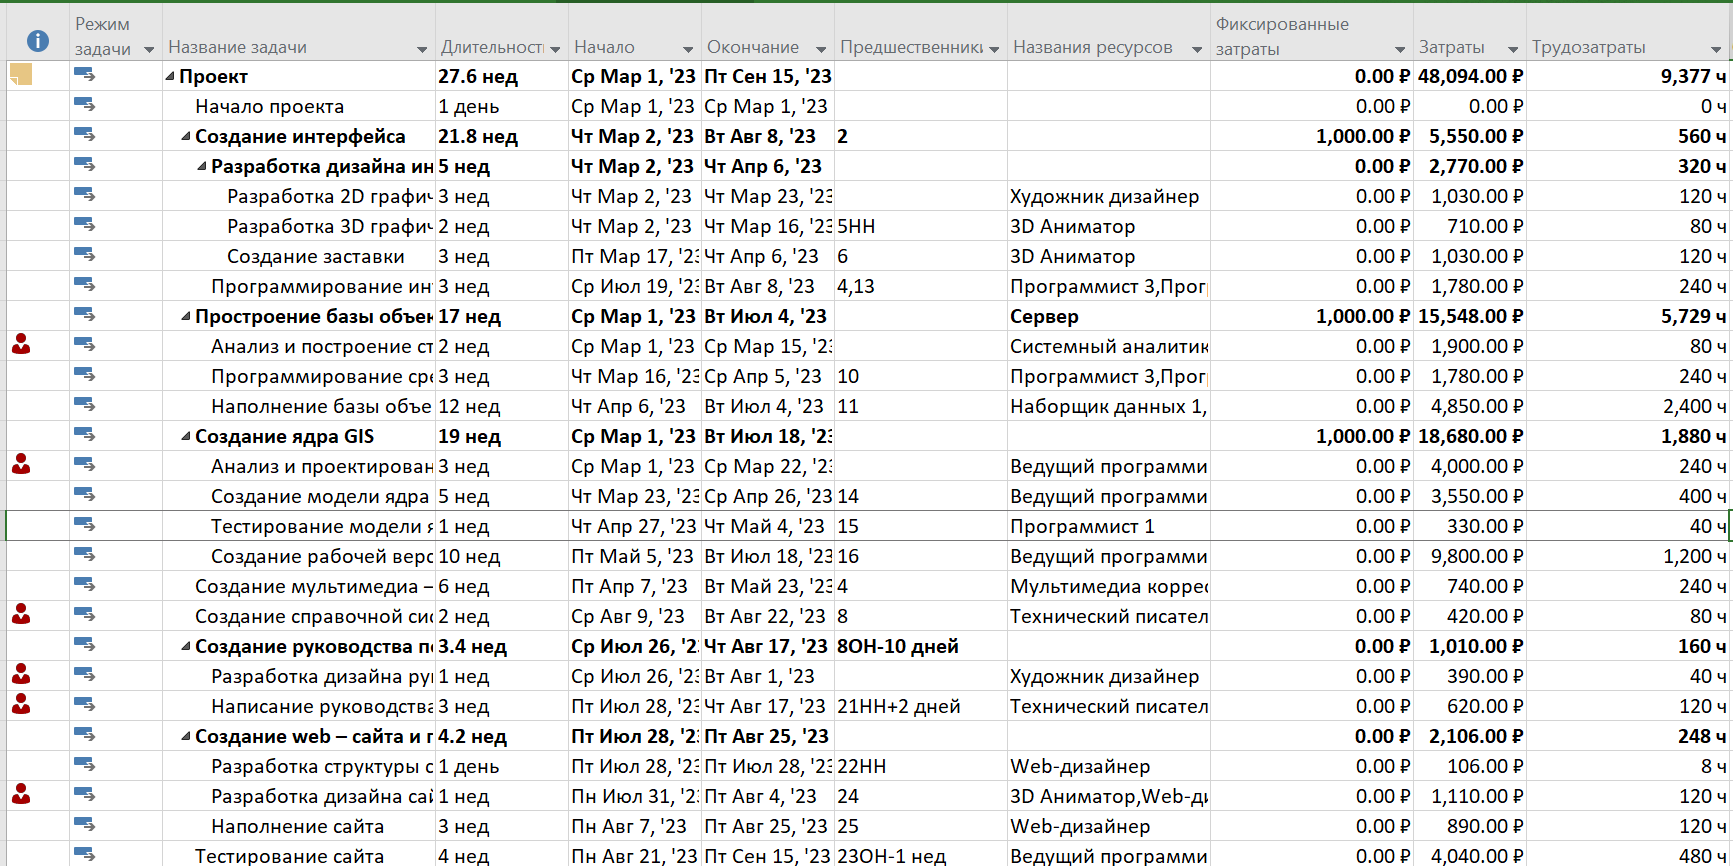
\includegraphics[width=\linewidth]{inc/new.png}
	\end{center}
	\captionsetup{justification=centering}
	\caption{Итоговый результат}
\end{figure}
\FloatBarrier

Из результата видно, что рядом с некоторыми записями в таблице появился красный маркер, который указывает на неправильное планирование ресурсов.
Это связано с тем, что некоторые ресурсы используются одновременно, соответственно, получается перерасход ресурса на определенном периоде.
На вкладке \textit{Вид} -> \textit{Лист Ресурсов} можно посмотреть подробности того, какие именно ресурсы используются неправильно:

\FloatBarrier
\begin{figure}[h]	
	\begin{center}
		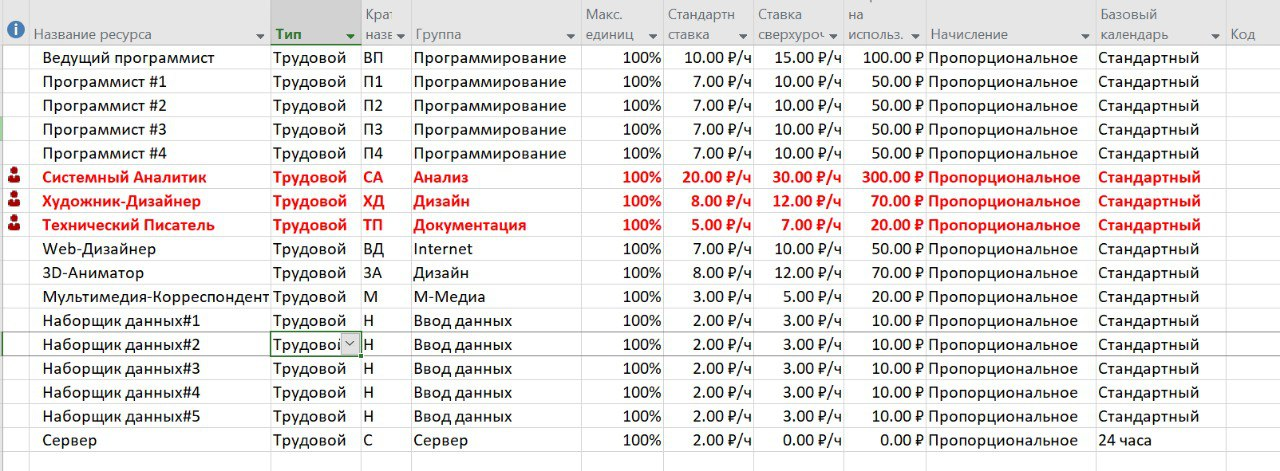
\includegraphics[width=\linewidth]{inc/2-3.jpeg}
	\end{center}
	\captionsetup{justification=centering}
	\caption{Перерасход некоторых ресурсов}
\end{figure}
\FloatBarrier

Подробности по одному из проблемных ресурсов представлены на рисунке:
\FloatBarrier
\begin{figure}[h]	
	\begin{center}
		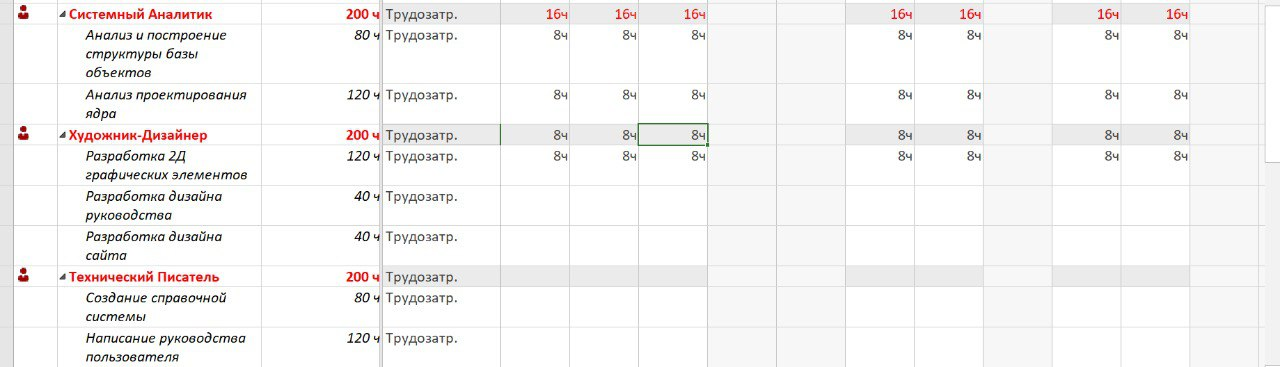
\includegraphics[width=\linewidth]{inc/2-4.jpeg}
	\end{center}
	\captionsetup{justification=centering}
	\caption{Конкретная информация по проблемному ресурсу}
\end{figure}
\FloatBarrier

Результаты сохранены в отдельном файле \textbf{task2.mpp}.
\newpage

\anonsection{Задание 3}
Требуется провести анализ затрат и трудозатрат по группам ресурсов.
Полные затраты проекта представлены на рисунке 6:
\FloatBarrier
\begin{figure}[h]	
	\begin{center}
		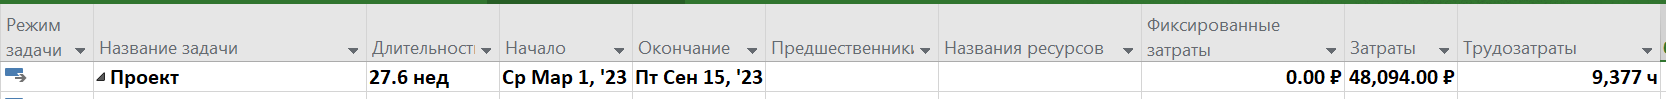
\includegraphics[width=\linewidth]{inc/res1.png}
	\end{center}
	\captionsetup{justification=centering}
	\caption{Полные затраты проекта}
\end{figure}
\FloatBarrier

Для анализа затрат и трудозатрат по группам ресурсов удобнее всего использовать круговую диаграмму -- с помощью неё можно наглядно посмотреть относительные величины затрат ресурсов.
На рисунке представлена диаграмма для затрат:
\FloatBarrier
\begin{figure}[h]	
	\begin{center}
		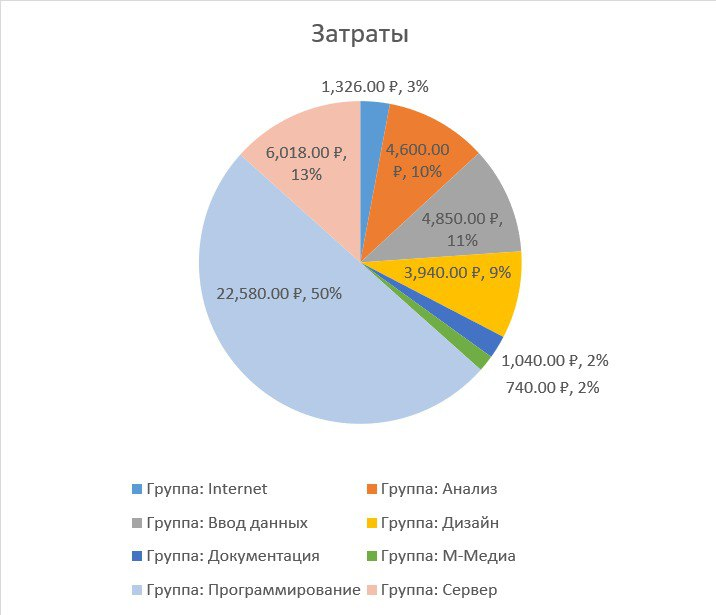
\includegraphics[width=\linewidth, height=13cm]{inc/4-1.jpg}
	\end{center}
	\captionsetup{justification=centering}
	\caption{Распределение затрат по группам ресурсов}
\end{figure}
\FloatBarrier

\newpage
Круговая диаграмма для трудозатрат представлена на рисунке:
\FloatBarrier
\begin{figure}[h]	
	\begin{center}
		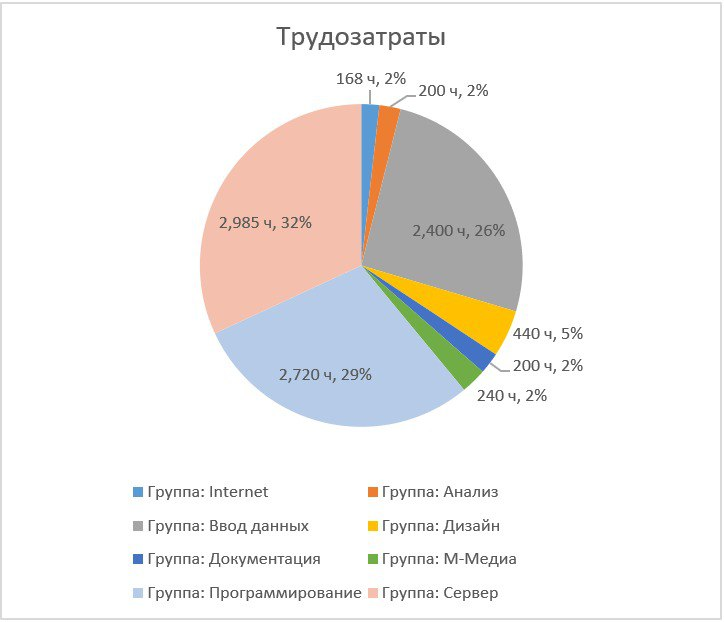
\includegraphics[width=\linewidth]{inc/4-2.jpg}
	\end{center}
	\captionsetup{justification=centering}
	\caption{Распределение трудозатрат по группам ресурсов}
\end{figure}
\FloatBarrier

По этим диаграммам можно сделать следующие выводы:
\begin{enumerate}
	\item Группа затрат \textbf{программирование} является наиболее существенной -- 50\% всех затрат и 29\% всех трудозатрат уходят именно на эти ресурсы. Это значит, что для оптимизации бюджета и сроков в первую очередь нужно обратить внимание именно на эту группу.
	\item \textbf{Сервер} занимает 32\% всех трудозатрат из-за того, что он работает 24 часа. Тем не менее, ресурс не является человеческим, что лишь увеличивает долю трудозатрат программистов среди всего персонала. При этом сервер занимает лишь 13\% всех затрат. 
	\item \textbf{Дизайн}, \textbf{документация} и \textbf{мультимедия} оказывают незначительное влияние на бюджет и трудозатраты проекта.
	\item \textbf{Анализ} при незначительных трудозатратах потребляет 10\% затрат команды, поэтому в случае перерасхода бюджета стоит обратить внимание на ставку аналитиков.
	\item Группа \textbf{набора данных} имеет 26\% трудозатрат проекта, но всего 11\% затрат, соответственно, для ускорения проекта можно увеличить команду наборщиков без сильных нагрузок по бюджету.
\end{enumerate}

\anonsection{Выводы}
В этой лабораторной работе под задачи были созданы и выделены ресурсы.
Выяснилось, что три ресурса оказываются перегружены.
Для решения этой проблемы существует несколько путей:
\begin{enumerate}
	\item Добавить больше ресурсов, что приведёт к большим расходам.
	\item Увеличить сроки выполнения заданий, из-за чего проект ещё больше растянется по времени. Требуется закончить проект до 1 сентября, тогда как сейчас сроки -- до 15 сентября, то есть такой подход не может быть применен на практике.
	\item Изменить последовательность выполнения задач.
	\item Изменить применение ресурсов для выполнения задач: например, выделить больше программистов на одну работу.
\end{enumerate}

Текущие затраты вписываются в бюджет, но по срокам возникают проблемы: нужно ускорить разработку как минимум на две недели.

В рамках изучения Microsoft Project были изучены темы создания ресурсов, выделение ресурсов задачам и построение графиков для последующего анализа.



